\chapter{Tính toán trục}
\section{Chọn vật liệu và tính sơ bộ}
Vì chưa biết chiều dài trục nên ta thiết kế sơ bộ để xác định đường kính trục theo moment xoắn. 
Chọn vật liệu chế tạo trục là thép C45 tôi cải thiện. Do trục bánh răng trong hộp giảm tốc là chi tiết máy rất quan trọng.

Tra bảng thông số vật liệu ta có thông số cơ tính của vật liệu như sau:
\begin{itemize}
    \item Loại thép: 45
    \item Nhiệt luyện: tôi cải thiện
    \item Độ rắn: $HB_1 = 260 \, \text{HB}$
    \item Giới hạn bền: $\sigma_b = 850 \, \text{MPa}$
    \item Giới hạn chảy: $\sigma_{ch} = 650 \, \text{MPa}$
\end{itemize}
Chọn ứng suất xoắn cho phép $[\tau] = 20 \, \text{MPa}$ \\
Xác định sơ bộ đường kính trục:
\[
d_1 \geq \sqrt[3]{\frac{T_1}{0.2[\tau]}} = \sqrt[3]{\frac{65914.47}{0.2 \cdot 20}} = 25.44 \text{mm}
\]
\[
d_2 \geq \sqrt[3]{\frac{T_2}{0.2[\tau]}} = \sqrt[3]{\frac{321365.99}{0.2 \cdot 20}} = 37.69 \text{mm}
\]
Tra bảng 10.2 tài liệu [2], ta chọn sơ bộ đường kính trục và bề rộng ổ lăn theo tiêu chuẩn:
\begin{itemize}
    \item Trục I: $d_1 = 25.44 \, \text{mm}$; $b_{o1} = 19 \, \text{mm}$
    \item Trục II: $d_2 = 35 \, \text{mm}$; $b_{o2} = 25 \, \text{mm}$  
\end{itemize}
\section{Xác định khoảng cách giữa các ổ lăn và điểm đặt lực}
\subsection{Trục I}
Theo bảng 10.3 tài liệu [2], ta có:
\begin{itemize}
    \item $k_1 = 8$ mm: Khoảng cách từ mặt mút của chi tiết quay đến thành trong của hộp hoặc khoảng cách giữa các chi tiết quay
    \item $k_2 = 10$ mm: Khoảng cách từ mặt mút ổ đến thành trong của hộp
    \item $k_3 = 10$ mm: Khoảng cách từ mặt mút của chi tiết quay đến nắp ổ
    \item $h_n = 15$ mm: Chiều cao nắp ổ và đầu bu lông
    \item Chọn sơ bộ chiều dài mayơ bánh răng trụ dẫn: $l_{m13}$ = bề dày bánh răng $b_w$ = 70 mm
    \item Chọn sơ bộ chiều dài mayơ bánh đai: $l_{m12} = (1.2\div 1.5)d_1 = 30 \div 37.5$. Chọn $l_{m22}=36$ mm 
    \item $l_{13} = 0.5(l_{m13} + b_{o1}) + k_1 + k_2 = 0.5(70 + 21) + 10 + 8 = 63.5 \, \text{mm}$
    \item $l_{11} = 2l_{13} = 2 \cdot 63.5 = 127 \, \text{mm}$
 
    \item $l_{12} = 0.5(l_{m12} + b_{o1}) + k_3 + h_n = 0.5(50 + 21) + 10 + 15 = 75.5 \, \text{mm}$
\end{itemize}

\subsection{Trục II}
Theo bảng 10.3 tài liệu [2], ta có:
\begin{itemize}
    \item $k_1 = 8$ mm: Khoảng cách từ mặt mút của chi tiết quay đến thành trong của hộp hoặc khoảng cách giữa các chi tiết quay
    \item $k_2 = 10$ mm: Khoảng cách từ mặt mút ổ đến thành trong của hộp
    \item $k_3 = 10$ mm: Khoảng cách từ mặt mút của chi tiết quay đến nắp ổ
    \item $h_n = 15$ mm: Chiều cao nắp ổ và đầu bu lông
    \item $l_{m23}$ = bề dày bánh răng $b_w$ = 64 mm
    \item $l_{m22} = (1.2\div 1.5)d_1 = 45.25 \div 57$. Chọn $l_{m22}=57$ mm
    \item $l_{23} = 0.5(l_{m13} + b_{o1}) + k_1 + k_2 = 64.5 \, \text{mm}$
    \item $l_{21} = 0.5(l_{m23} + b_{o2}) + k_1 + k_2 = 140.5 \, \text{mm}$
    \item $l_{22} = 2l_{21}$ = 
\end{itemize}

\section{Phân tích lực tác dụng}
\subsection{Trục I}
\begin{itemize}
    \item Lực vòng: $F_{t1}$ = 2471.8 N
    \item Lực dọc trục: $F_{a1}$ = 756.18 N
    \item Lực hướng tâm: $F_{r1}$ = 940.82 N 
    \item Lực do bộ truyền đai: $F_d$ = 474.74 N
\end{itemize}
\subsection{Trục II}
\begin{itemize}
    \item Lực vòng: $F_{t2}$ = 2471.8 N
    \item Lực dọc trục: $F_{a2}$ = 940.82 N
    \item Lực hướng tâm: $F_{r2}$ = 756.18 N 
    \item Lực nối trục: $F_{nt}$ = 1483.23 N
\end{itemize}
\section{Tính momen tương đương và đường kính trục}
\subsection{Trục I}
Moment do lực dọc trục tạo ra:
\[
    M_{a1} = F_{a1} \cdot \frac{d_1}{2} 
           = 756.177 \cdot \frac{53.33}{2} 
           = 20163.47\ \text{Nmm}
\]
\[
    \left\{
    \begin{array}{l}
        \sum F_X = 0 \\
        \sum F_Y = 0 \\
        \sum M_{Y/A} = 0 \\
        \sum M_{X/A} = 0
    \end{array}
    \right.
    \Leftrightarrow
    \left\{
    \begin{array}{l}
        -F_{dx} - R_{BX} + F_{t1} - R_{DX} = 0 \\
        -F_{dy} - R_{BY} + F_{r1} - R_{DY} = 0  \\
        -52 R_{BX} + 116.5 F_{t1} - 181R_{DX} = 0 \\
        -52 R_{BY} + 116.5 F_{r1} - M_{a1} - 181 R_{DY} = 0
    \end{array}
    \right.
    \Leftrightarrow
    \left\{
    \begin{array}{l}
        R_{BX} = 1879.31\ \text{N} \\
        R_{BY} = 454.31\ \text{N} \\
        R_{DX} = 1051.05\ \text{N} \\
        R_{DY} = 363.63\ \text{N}
    \end{array}
    \right.
\]
\begin{figure}[H]
    \centering
    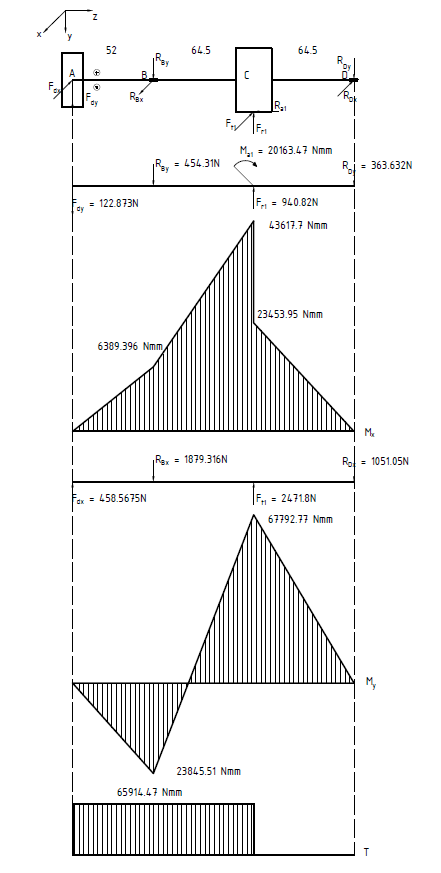
\includegraphics[width=0.8\textwidth]{pictures/momen1.png}
\end{figure}
\[
    M_A^{td} 
    = \sqrt{M_{X/A}^2 + M_{Y/A}^2 + 0.75 \cdot T_A^2} 
    = \sqrt{0.75 \cdot 65914.47^2}  
    = 57083.6\ \text{Nmm}
\]

\[
    M_B^{td} 
    = \sqrt{M_{X/B}^2 + M_{Y/B}^2 + 0.75 \cdot T_B^2} 
    = \sqrt{6389.396^2 + 23845.51^2 + 0.75 \cdot 65914.47^2} 
    = 62193.01\ \text{Nmm}
\]

\[
    M_C^{td} 
    = \sqrt{M_{X/C}^2 + M_{Y/C}^2 + 0.75 \cdot T_C^2} 
    = \sqrt{43617.7^2 + 67792.77^2 + 0.75 \cdot 65914.47^2} 
    = 98777.03\ \text{Nmm}
\]

\[
    M_D^{td} 
    = \sqrt{M_{X/D}^2 + M_{Y/D}^2 + 0.75 \cdot T_D^2} 
    = 0 
\]
$\Rightarrow$ Vị trí nguy hiểm là vị trí C.
\[
    d_C \ge \sqrt[3]{\frac{M_C^{td}}{0.1 \cdot \sigma}} 
        = \sqrt[3]{\frac{98777.03}{0.1 \cdot 67}} 
        = 24.5\ \text{mm}
\]
Tại ví trí C có lắp bánh răng, do đó ta tăng đường kính trục thêm 5\% = 25.7 mm. \\
Căn cứ theo kết cấu của trục và bánh răng dẫn, thiết kế trục dẫn 1 với bánh răng liền trục, đường kính các tiết diện còn lại chọn để thỏa mãn yêu cầu về lắp ráp và thỏa mãn dãy kích thước tiêu chuẩn: 
\begin{itemize}
    \item $d_A$ = 22 mm
    \item $d_B$ = 30 mm
    \item $d_D$ = 30 mm
\end{itemize}

\subsection{Trục II}
Moment do lực dọc trục tạo ra:
\[
    M_{a2} = F_{a2} \cdot \frac{d_2}{2} 
           = 756.177 \cdot \frac{266.67}{2} 
           = 100825\ \text{Nmm}
\]
\[
    \left\{
    \begin{array}{l}
        \sum F_X = 0 \\
        \sum F_Y = 0 \\
        \sum M_{Y/A} = 0 \\
        \sum M_{X/A} = 0
    \end{array}
    \right.
    \Leftrightarrow
    \left\{
    \begin{array}{l}
        R_{AX} - F_{t2} - R_{CX} + F_{nt} = 0 \\
        -R_{AY} - F_{r2} + R_{CY} \\
        -76 F_{t2} - 140.5 R_{CX} + 205 F_{nt} = 0 \\
        -76 F_{r2} + 140.5 R_{CY} - M_{a1} = 0
    \end{array}
    \right.
    \Leftrightarrow
    \left\{
    \begin{array}{l}
        R_{AX} = 1815.8\ \text{N} \\
        R_{AY} = 287.235\ \text{N} \\
        R_{CX} = 827.235\ \text{N} \\
        R_{CY} = 1228.49\ \text{N}
    \end{array}
    \right.
\]
\begin{figure}[H]
    \centering
    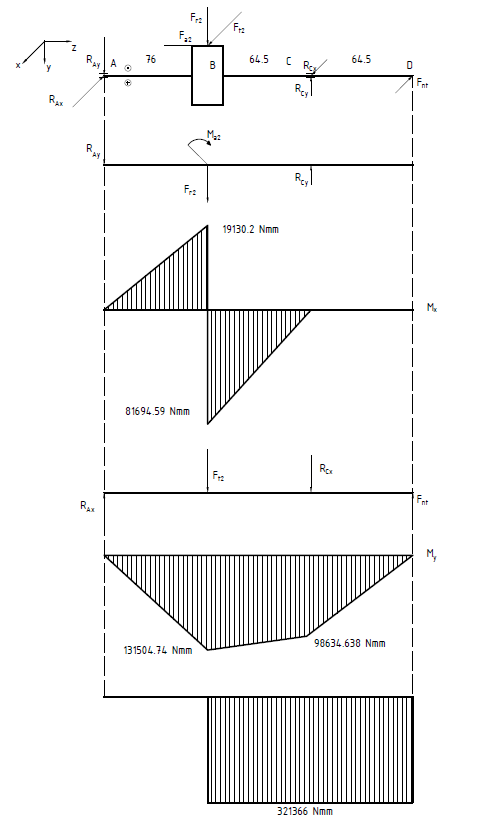
\includegraphics[width=0.9\textwidth]{pictures/momen2.png}
\end{figure}
\[
    M_A^{td} 
    = \sqrt{M_{X/A}^2 + M_{Y/A}^2 + 0.75 \cdot T_A^2} 
    = 0
\]

\[
    M_B^{td} 
    = \sqrt{M_{X/B}^2 + M_{Y/B}^2 + 0.75 \cdot T_B^2} 
    = \sqrt{81694.59^2 + 131504.74^2 + 0.75 \cdot 321366^2} 
    = 318472.26\ \text{Nmm}
\]

\[
    M_C^{td} 
    = \sqrt{M_{X/C}^2 + M_{Y/C}^2 + 0.75 \cdot T_C^2} 
    = \sqrt{98634.638^2 + 0.75 \cdot 321366^2} 
    = 295272.54\ \text{Nmm}
\]

\[
    M_D^{td} 
    = \sqrt{M_{X/D}^2 + M_{Y/D}^2 + 0.75 \cdot T_D^2} 
    = \sqrt{0.75 \cdot 321366^2} 
    = 278311.12\ \text{Nmm}
\]
$\Rightarrow$ Vị trí nguy hiểm là vị trí B.
\[
    d_B \ge \sqrt[3]{\frac{M_B^{td}}{0.1 \cdot \sigma}} 
        = \sqrt[3]{\frac{318472.26}{0.1 \cdot 67}} 
        = 36.22\ \text{mm}
\]
Tại ví trí B có lắp bánh răng, do đó ta tăng đường kính trục thêm 5\% = 38 mm. \\
Như vậy, để thỏa mãn dãy kích thước tiêu chuẩn và yêu cầu lắp ráp, ta chọn:
\begin{itemize}
    \item $d_A$ = 40 mm
    \item $d_B$ = 45 mm     
    \item $d_C$ = 40 mm
    \item $d_D$ = 36 mm
\end{itemize}

\section{Tính toán và kiểm nghiệm then}
\subsection{Xác định ứng suất dập cho phép và ứng suất cắt cho phép của then tại các vị trí lắp ráp}
\subsubsection{Mối ghép then tại tiết diện lắp bánh đai trên trục I}
\begin{itemize}
    \item Do bánh đai được chế tạo từ gang ở chế độ tải trọng tĩnh, ta có ứng suất dập cho phép của then $[\sigma_d] = 80 \, MPa$ (Bảng 9.5, Trịnh Chất tập 1).
    \item Ứng suất cắt cho phép của then $[\tau_c] = 60 \dots 90 \, MPa$, ta chọn $[\tau_c] = 60 \, MPa$.
    \item Dựa vào đường kính trục và bảng 9.1a [2], ta chọn then bằng cho mối ghép trên và có kích thước sau:
    \begin{table}[h!]
    \centering
    \begin{tabular}{|c|c|c|c|c|}
    \hline
    $\mathbf{d}$ & $\mathbf{b}$ & $\mathbf{h}$ & $\mathbf{t_1}$ & $\mathbf{t_2}$ \\
    \hline
    22 & 8 & 7 & 4 & 2.8 \\
    \hline
    \end{tabular}
    \end{table}
\end{itemize}
\subsubsection{Các mối ghép then trên trục II}
\begin{itemize}
    \item Do bánh răng và nối trục đều được chế tạo từ thép nên ở chế độ tải trọng tĩnh, ta có ứng suất dập cho phép của then $[\sigma_d] = 150 \, MPa$ (Bảng 9.5, Trịnh Chất tập 1).
    \item Ứng suất cắt cho phép của then $[\tau_c] = 60 \dots 90 \, MPa$, ta chọn $[\tau_c] = 60 \, MPa$.
    \item Dựa vào đường kính trục và bảng 9.1a (Trịnh Chất, tập 1), ta chọn then bằng cho mối ghép trên và có kích thước sau:
    \begin{itemize}
        \item Tại vị trí lắp bánh răng:
        \begin{table}[h!]
        \centering
        \begin{tabular}{|c|c|c|c|c|}
        \hline
        $\mathbf{d}$ & $\mathbf{b}$ & $\mathbf{h}$ & $\mathbf{t_1}$ & $\mathbf{t_2}$ \\
        \hline
        45 & 14 & 9 & 5.5 & 3.8 \\
        \hline
        \end{tabular}
        \end{table}
        \item Tại vị trí lắp nối trục:
        \begin{table}[h!]
        \centering
        \begin{tabular}{|c|c|c|c|c|}
        \hline
        $\mathbf{d}$ & $\mathbf{b}$ & $\mathbf{h}$ & $\mathbf{t_1}$ & $\mathbf{t_2}$ \\
        \hline
        36 & 10 & 8 & 5 & 3.3 \\
        \hline
        \end{tabular}
        \end{table}
    \end{itemize}
\end{itemize}
\subsection{Tính toán kiểm nghiệm mối ghép then theo độ bền dập và độ bền cắt}
\begin{itemize}
    \item Chọn chiều dài then $l_t$ theo tiêu chuẩn, nhỏ hơn chiều dày may-ơ bánh răng hoặc bánh đai khoảng $5 \rightarrow 10mm$.
    \item Đối với then bằng 2 đầu tròn tại vị trí lắp bánh răng trên trục II, chiều dài làm việc của then $l_{lv} = l_t - b$. Giá trị kiểm định thu được:
\end{itemize}

\begin{table}[h!]
\centering
\begin{tabular}{|c|c|c|c|c|c|c|c|c|c|c|}
\hline
\textbf{Tiết diện} & $\mathbf{b}$ & $\mathbf{h}$ & $\mathbf{l_t}$ & $\mathbf{l_{lv}}$ & $\mathbf{t_1}$ & $\mathbf{t_2}$ & $\mathbf{\sigma_d}$ & $\mathbf{\tau_c}$ & $\mathbf{[\sigma_d]}$ & $\mathbf{[\tau_c]}$ \\
\hline
Trục I - A & 8 & 7 & 28 & 28 & 4 & 2.8 & 71,33600649 & 26,75100244 & 80 & 60 \\
\hline
Trục II - B & 14 & 9 & 56 & 47 & 5,5 & 3,8 & 86,82633975 & 16,46378429 & 150 & 60 \\
\hline
Trục II - D & 10 & 8 & 45 & 45 & 5 & 3,3 & 132,2493786 & 47,6097763 & 150 & 60 \\
\hline
\end{tabular}
\end{table}

\noindent Như vậy các then đều thỏa mãn độ bền dập và độ bền cắt.
% \begin{itemize}
%     \item Dựa vào bảng 9.1 là tài liệu [2], chọn kích thước then BXH theo tiết diện lớn nhất của trước.
%     \item Chọn chiều dài $l$, theo tiêu chuẩn của then, nhỏ hơn chiều dài mayơ $l_m = 5 \div 10$ mm.
%     \item Kiểm nghiệm then theo độ bền đập và độ bền cắt then băng
%     \[
%     \sigma_d = \frac{2T}{d l_w (h - t_1)} \leq [\sigma_d] \quad \tau_c = \frac{2T}{d l_w b} \leq [\tau_c]
%     \]
%     Với
%     \[
%     [\sigma_d] = 150 \, \text{MPa}, \text{tra theo bảng 9.5 tài liệu \cite{2}}
%     \]
%     \[
%     [\tau_c] = 60 \div 90 \, \text{MPa}
%     \]
%     $l_w = l - b$: chiều dài làm việc của then băng 2 đầu tròn
% \end{itemize}
% \textbf{Bảng thông số:}
% \begin{center}
% \begin{tabular}{|l|c|c|c|c|c|c|c|c|c|c|c|}
% \hline
% \textbf{Trục} & \textbf{Đường kính} & \textbf{Mặt cắt} & $l_m$ & $l$ & $l_w$ & $b$ & $h$ & $t_1$ & $\sigma_d$ & $\tau_c$ & $T$ \\
% \hline
% \multirow{2}{*}{\textbf{I}} & 28 & 12 & 45 & 40 & 32 & 8 & 7 & 4 & 107,4 & 40,3 & 1443308,115 \\
% \cline{2-12}
% & 35 & 13 & 70 & 65 & 55 & 10 & 8 & 5 & 49,97 & 15,0 & 1443308,115 \\
% \hline
% \multirow{2}{*}\textbf{II} & 55 & 22 & 75 & 70 & 54 & 16 & 10 & 6 & 101,1 & 25,3 & 600394,168 \\
% \cline{2-12}
% & 46 & 23 & 75 & 70 & 56 & 14 & 9 & 5,5 & 127,6 & 31,9 & 600394,168 \\
% \hline
% \end{tabular}
% \end{center}

% $\Rightarrow$ Các mặt cắt đều thỏa điều kiện bền đập và căng bền đảm bảo an toàn cho phép.

\section{Kiểm nghiệm độ bền trục}
\noindent Ứng suất bền giới hạn của thép C45 tôi là $\sigma_b = 600 \, MPa$, giới hạn mỏi của vật liệu được tính theo công thức:
$$ \sigma_{-1} = 0.436 \cdot \sigma_b = 261.6 \, MPa $$
$$ \tau_{-1} = 0.58 \cdot \sigma_{-1} = 151.73 \, MPa $$

\noindent Chọn hệ số an toàn $[s] = 2$, ta lần lượt kiểm nghiệm trục theo độ bền mỏi và độ bền tĩnh:

\subsection{Độ bền mỏi}
Hệ số an toàn:
\[
s = \frac{s_0 s_\tau}{\sqrt{s_0^2 + s_\tau^2}} \geq [s]
\]
\begin{itemize}
    \item Với hệ số an toàn cho phép $[s] = 1.5 \div 2.5$, khi tăng độ căng $[s] = 2.5 \div 3$, nhưng vậy không cần kiểm nghiệm về độ căng.
    \item $s_0, s_\tau$ hệ số an toàn chi xét riêng ứng suất pháp, ứng suất tiếp
    \[
    s_0 = \frac{K_0 \sigma_a + \psi_0 \sigma_m}{\varepsilon_\beta \sigma}, \quad s_\tau = \frac{K_\tau \tau_a + \psi_\tau \tau_m}{\varepsilon_\tau \tau}
    \]
    \item $\sigma_{-1}, \tau_{-1}$ giới hạn mỏi của vật liệu tính theo công thức:
    \[
    \sigma_{-1} = (0.4 \div 0.5) \sigma_b = 240 \div 300 \, \text{MPa}, \text{ chọn } \sigma_{-1} = 280 \, \text{MPa}
    \]
    \[
    \tau_{-1} = (0.22 \div 0.25) \sigma_b = 132 \div 150 \, \text{MPa}, \text{ chọn } \tau_{-1} = 140 \, \text{MPa}
    \]
    \[
    \sigma_b = 600 \, \text{MPa}: \text{giới hạn bền của thép 45 thường hóa}
    \]
    Theo bảng 10.8 tài liệu [1], $K_0 = 1.75$, $K_\tau = 1.5$
    \item $\sigma_a, \sigma_m, \tau_a, \tau_m$: biên độ và giá trị của ứng suất. Vì tất cả các trục của hợp giảm tốc đều quay nên ứng suất thay đổi theo chu kỳ đối xứng: $\sigma_m = 0$, $\sigma_a = \sigma_{\text{max}} = \frac{M}{W}$, với $M$ là moment uốn thương trường, $W$ là moment chóng uốn
    \item Đo trực quy 1 chiều nên ứng suất xoắn thay đổi theo chu kỳ mạch động
\end{itemize}
\[
\tau_a = \tau_m = \frac{T_{\text{max}}}{2}, \quad \text{với } W_0 \text{ là moment chống xoắn, } T \text{ là moment xoắn}
\]
\begin{itemize}
    \item $\psi_\sigma = 0.05; \psi_\tau = 0$ hệ số xét đến ảnh hưởng của ứng suất trung bình đến độ bền mỏi của vật liệu
    \item $\varepsilon_\sigma, \varepsilon_\tau$: hệ số kích thước (bảng 10.3 tài liệu [1])
    \item $\beta = 1.7$: hệ số tăng bề mặt (bảng 10.5 tài liệu [1])
\end{itemize}
\textbf{Bảng kết quả tính toán kiểm nghiệm trục theo độ bền mỏi}
\begin{center}
\begin{tabular}{|l|c|c|c|c|c|c|c|c|}
\hline
\textbf{Trục} & \textbf{Tiết diện} & $W$ & $ W_0 $ & $\varepsilon_\tau$ & $\varepsilon_\sigma$ & $s_\sigma$ & $s_\tau$ & $s$ \\
\hline
\multirow{4}{*}{\textbf{I}} & A & 6283.18 & 1855.09 & 0.92 & 0.89 & 21.89 & 3.58 & 3.53 \\
\cline{2-9}
& B & 7611.29 & 5301.44 & 0.92 & 0.89 & 24.34 & 10.22 & 9.43 \\
\cline{2-9}
& C & 6283.18 & 41006.52 & 0.85 & 0.78 & 11.71 & 69.6 & 11.55 \\
\cline{2-9}
& D & 3913.08 & 5301.44 & 0.92 & 0.89 & 13.63 & 10.22 & 8.18 \\
\hline
\multirow{4}{*}{\textbf{II}} & A & 6283.18 & 12566.37 & 0.88 & 0.81 & 4.3 & 4.54 & 3.13 \\
\cline{2-9}
& B & 7611.29 & 16557.47 & 0.85 & 0.78 & 4.46 & 5.76 & 3.53 \\
\cline{2-9}
& C & 6283.18 & 12566.47 & 0.88 & 0.81 & 3.91 & 4.54 & 2.96 \\
\cline{2-9}
& D & 3913.08 & 8493.52 & 0.88 & 0.81 & 2.68 & 3.07 & 2.02 \\
\hline
\end{tabular}
\end{center}
Như vậy tất cả tiết diện của 2 trục đều thỏa mãn độ bền mỏi.
\subsection{Độ bền tĩnh}
Để đề phòng trục bị biến dạng dẻo quá lớn hoặc bị gãy khi bị quá tải đột ngột ta cần kiểm nghiệm trục theo độ bền tĩnh:

\begin{itemize}
    \item Công thức thực nghiệm cơ dạng: $\sigma_d = \sqrt{\sigma^2 + 3\tau^2} \leq [\sigma_d]_t$
\end{itemize}

Trong đó:
\[
\sigma = \frac{M}{W} = \sigma_a; \quad \tau = \frac{T}{W_0} = 2\tau_a; \quad [\sigma_d]_t \approx 0.8\sigma_{ch} = 0.8340 = 272 \, \text{MPa}
\]
\textbf{Bảng kiểm nghiệm trục theo độ bền tĩnh}
\begin{center}
\begin{tabular}{|c|c|c|c|c|}
    \hline
      & $\sigma$ & $\tau$ & $\sigma_{td}$ & $[\sigma]$ \\
    \hline
    \multirow{4}{*}{\textbf{I}} &9.085 & 35.35 & 75.83 & 272 \\
    \cline{2-5}
     & 8.171 & 12.43 & 46.56 & 272 \\
     \cline{2-5}
     & 15.72 & 1.61 & 48.82 & 272 \\
     \cline{2-5}
     & 14.59 & 12.43 & 46.56 & 272 \\
     \hline
     \multirow{4}{*}{\textbf{II}} & 44.29 & 25.57 & 62.64 & 272 \\
     \cline{2-5}
      & 41.28 & 19.41 & 53.24 & 272 \\
      \cline{2-5}
      & 48.74 & 25.57 & 65.86 & 272 \\
      \cline{2-5}
      & 71.12 & 37.84 & 96.71 & 272 \\
      \hline
\end{tabular}
\end{center}
Vậy các trục thỏa điều kiện độ bền tĩnh